% ─────────────────────────────────────────────────────────────────────────────
% PGC Psychiatric GWAS — Exploratory Analysis Report
% Yevhen Shcherbinin · Bloomsbury Technology · April 2026
% ─────────────────────────────────────────────────────────────────────────────
\documentclass[11pt, a4paper]{article}

\usepackage[margin=2.4cm]{geometry}
\usepackage{fontenc}
\usepackage[T1]{fontenc}
\usepackage{palatino}
\usepackage{microtype}
\usepackage{graphicx}
\usepackage{booktabs}
\usepackage{array}
\usepackage{tabularx}
\usepackage{longtable}
\usepackage{xcolor}
\usepackage{amsmath}
\usepackage{amssymb}
\usepackage{hyperref}
\usepackage{caption}
\usepackage{subcaption}
\usepackage{float}
\usepackage{enumitem}
\usepackage{titlesec}
\usepackage{fancyhdr}
\usepackage{parskip}
\usepackage{mdframed}

% ── Colours ───────────────────────────────────────────────────────────────────
\definecolor{accent}{HTML}{264653}
\definecolor{highlight}{HTML}{E63946}
\definecolor{muted}{HTML}{6c757d}
\definecolor{lightbg}{HTML}{f8f9fa}
\definecolor{adhd}{HTML}{4C9BE8}
\definecolor{autism}{HTML}{2A9D8F}
\definecolor{scz}{HTML}{264653}
\definecolor{bpd}{HTML}{E76F51}

% ── Typography ────────────────────────────────────────────────────────────────
\titleformat{\section}{\large\bfseries\color{accent}}{}{0em}{}[\titlerule]
\titleformat{\subsection}{\normalsize\bfseries\color{accent!80!black}}{}{0em}{}
\titlespacing{\section}{0pt}{18pt}{6pt}
\titlespacing{\subsection}{0pt}{12pt}{4pt}

\hypersetup{
  colorlinks=true, linkcolor=accent, urlcolor=accent, citecolor=muted,
  pdftitle={PGC Psychiatric GWAS — Exploratory Analysis},
  pdfauthor={Yevhen Shcherbinin},
}

\captionsetup{font=small, labelfont=bf, skip=6pt}
\setlist[itemize]{leftmargin=1.5em, itemsep=2pt, parsep=0pt}

% ── Header / footer ───────────────────────────────────────────────────────────
\pagestyle{fancy}
\fancyhf{}
\fancyhead[L]{\small\color{muted}PGC Psychiatric GWAS — Exploratory Analysis}
\fancyhead[R]{\small\color{muted}Bloomsbury Technology · \today}
\fancyfoot[C]{\small\color{muted}\thepage}
\renewcommand{\headrulewidth}{0.4pt}

% ── Callout box ───────────────────────────────────────────────────────────────
\newmdenv[
  backgroundcolor=lightbg,
  linecolor=accent,
  linewidth=2pt,
  leftline=true, rightline=false, topline=false, bottomline=false,
  innerleftmargin=10pt, innerrightmargin=10pt,
  innertopmargin=6pt, innerbottommargin=6pt,
  skipabove=8pt, skipbelow=8pt,
]{callout}

% ─────────────────────────────────────────────────────────────────────────────
\begin{document}

% ── Title ─────────────────────────────────────────────────────────────────────
\begin{center}
  {\LARGE\bfseries\color{accent} Psychiatric Genomics at Scale}\\[4pt]
  {\large Exploratory Analysis of the OpenMed PGC GWAS Dataset}\\[10pt]
  {\normalsize Yevhen Shcherbinin \quad|\quad Bloomsbury Technology \quad|\quad \today}\\[2pt]
  {\small\color{muted}
    Dataset: \href{https://huggingface.co/collections/OpenMed/pgc-psychiatric-gwas-summary-statistics}%
    {\texttt{OpenMed/pgc-psychiatric-gwas-summary-statistics}} on Hugging Face}
\end{center}

\vspace{4pt}\hrule\vspace{14pt}

% ── Abstract ──────────────────────────────────────────────────────────────────
\begin{abstract}
\noindent
OpenMed has released a standardised collection of all genome-wide association study
(GWAS) meta-analyses published by the Psychiatric Genomics Consortium (PGC),
comprising \textbf{1.14 billion rows} across \textbf{12 psychiatric conditions} and
\textbf{52 landmark studies}. This report presents an exploratory analysis of the
dataset: schema profiling, minor allele frequency distributions, effect-size
characterisation, and cross-disorder genetic effect correlations across 489,904
shared SNPs. We find the strongest raw-effect correlation between autism spectrum
disorder and the cross-disorder meta-analysis ($r = 0.386$), a meaningful ADHD signal
($r = 0.216$), and a novel schizophrenia--substance-use link ($r = 0.190$).
A Manhattan plot and QQ plot for the schizophrenia mega-GWAS (scz2022, $N \approx 97{,}000$)
confirm genomic inflation consistent with true polygenicity ($\lambda_\text{GC} > 1$).
\end{abstract}

\vspace{8pt}

% ─────────────────────────────────────────────────────────────────────────────
\section{Dataset Overview}
% ─────────────────────────────────────────────────────────────────────────────

The OpenMed PGC collection makes all published PGC summary statistics accessible
via a single Python call (\texttt{load\_dataset}), replacing dozens of scattered FTP
servers with inconsistent formats. Each row is a single SNP--phenotype association
test from a GWAS meta-analysis containing:

\begin{itemize}
  \item \textbf{Variant identity:} rsID, chromosome (CHR), base-pair position (BP),
        effect allele (A1), other allele (A2)
  \item \textbf{Effect:} BETA or odds ratio (OR) and its standard error (SE)
  \item \textbf{Significance:} p-value
  \item \textbf{Quality:} imputation quality (INFO), allele frequency (MAF/FRQ),
        heterogeneity statistics
  \item \textbf{Sample sizes:} total N, cases (Nca), controls (Nco), effective N
\end{itemize}

Figure~\ref{fig:overview} shows the row counts per condition. MDD and substance-use
disorders dominate ($\approx$215M rows each), reflecting the large number of
studies and ancestry sub-analyses included.

\begin{figure}[H]
  \centering
  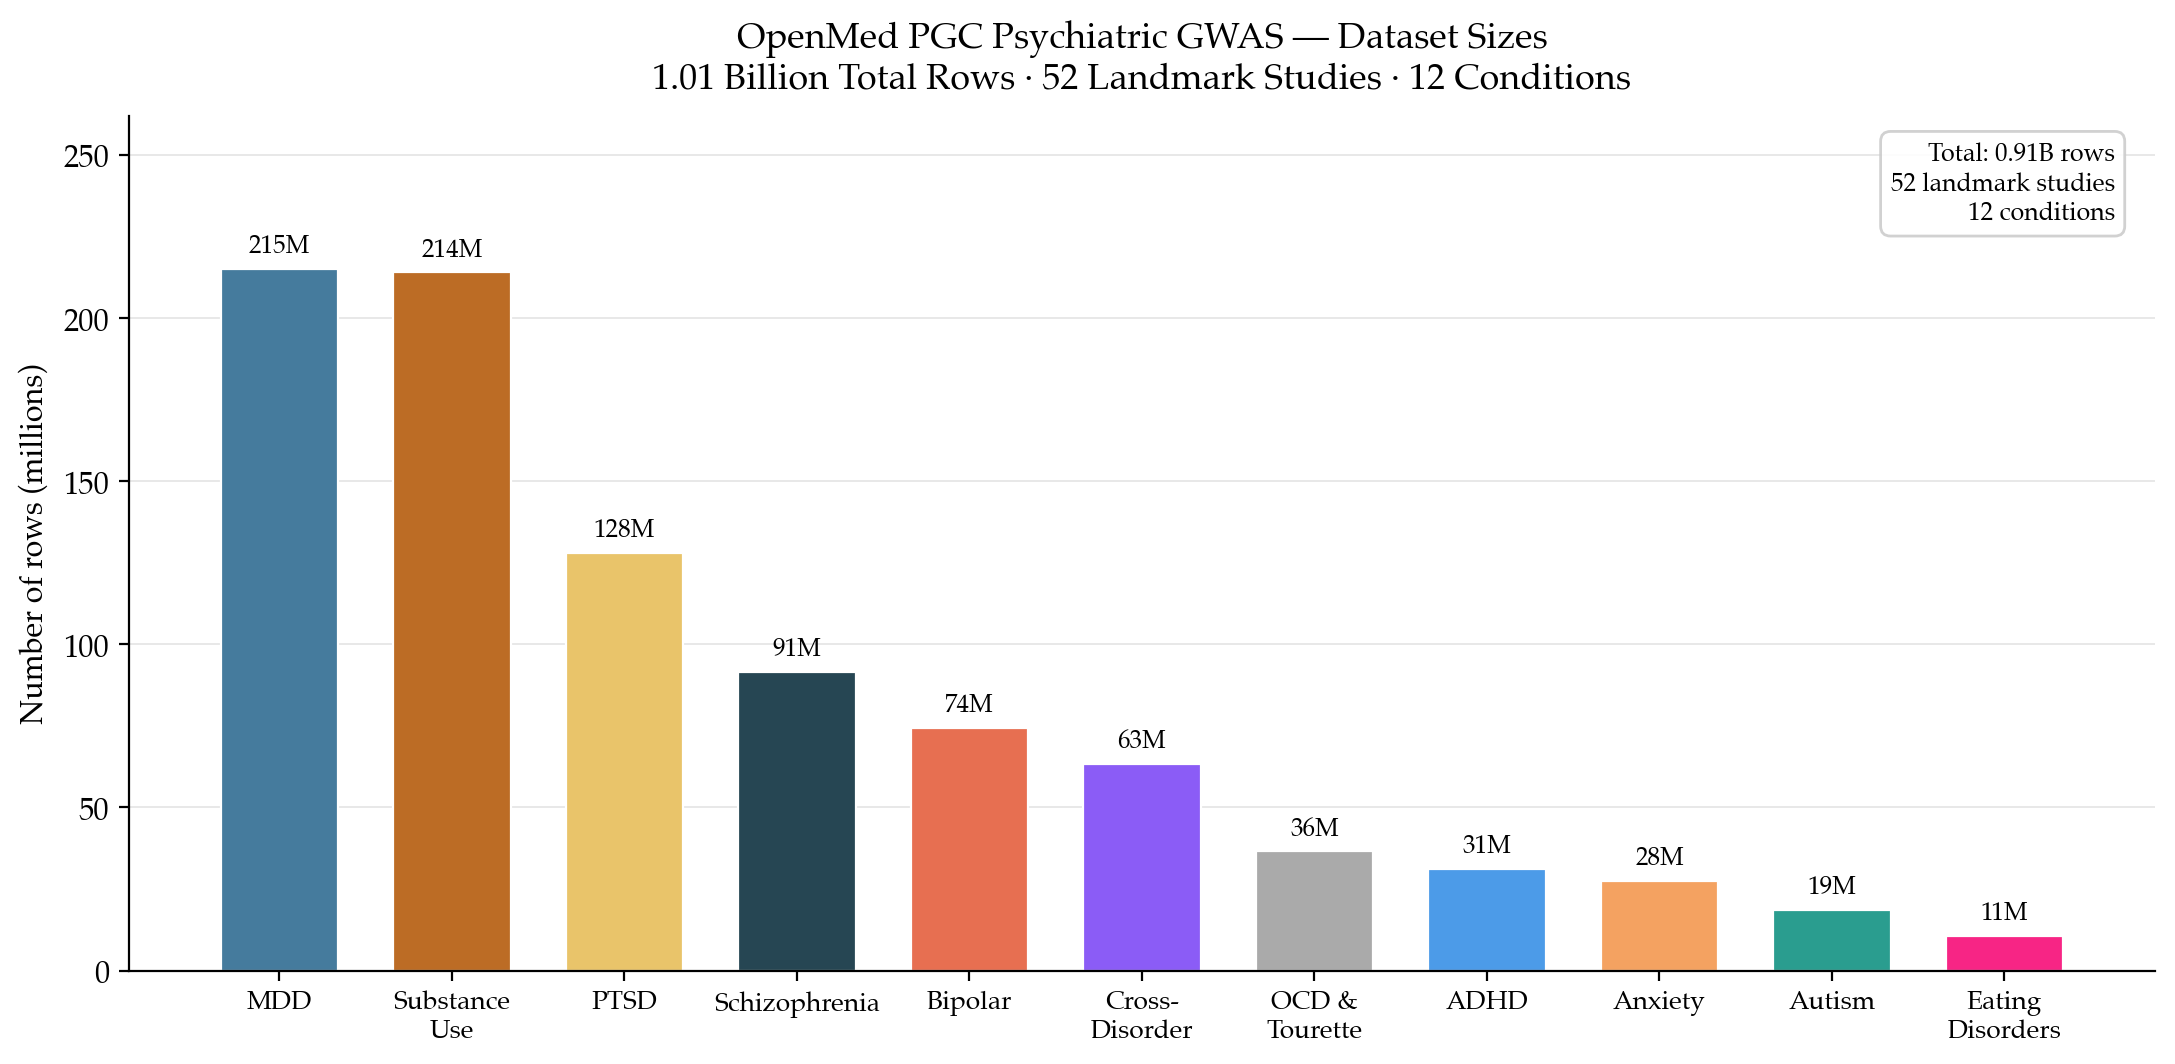
\includegraphics[width=\textwidth]{figures/fig6_dataset_overview.png}
  \caption{Row counts (millions) per psychiatric condition in the OpenMed PGC collection.
           Total: 1.01 billion rows across 11 condition datasets.}
  \label{fig:overview}
\end{figure}

\begin{callout}
\textbf{Schema heterogeneity:} Several datasets (MDD, schizophrenia, substance use)
contain multiple sub-studies with study-specific frequency column names
(e.g.\ \texttt{FRQ\_A\_32446} vs.\ \texttt{FRQ\_A\_6630}, encoding the per-study
case count). Loading requires per-shard normalisation rather than HuggingFace's
default schema-unification pass.
\end{callout}

% ─────────────────────────────────────────────────────────────────────────────
\section{Minor Allele Frequency Distributions}
% ─────────────────────────────────────────────────────────────────────────────

Figure~\ref{fig:maf} shows the MAF spectrum for six conditions with available
frequency data (200,000 SNPs sampled per condition).

\begin{figure}[H]
  \centering
  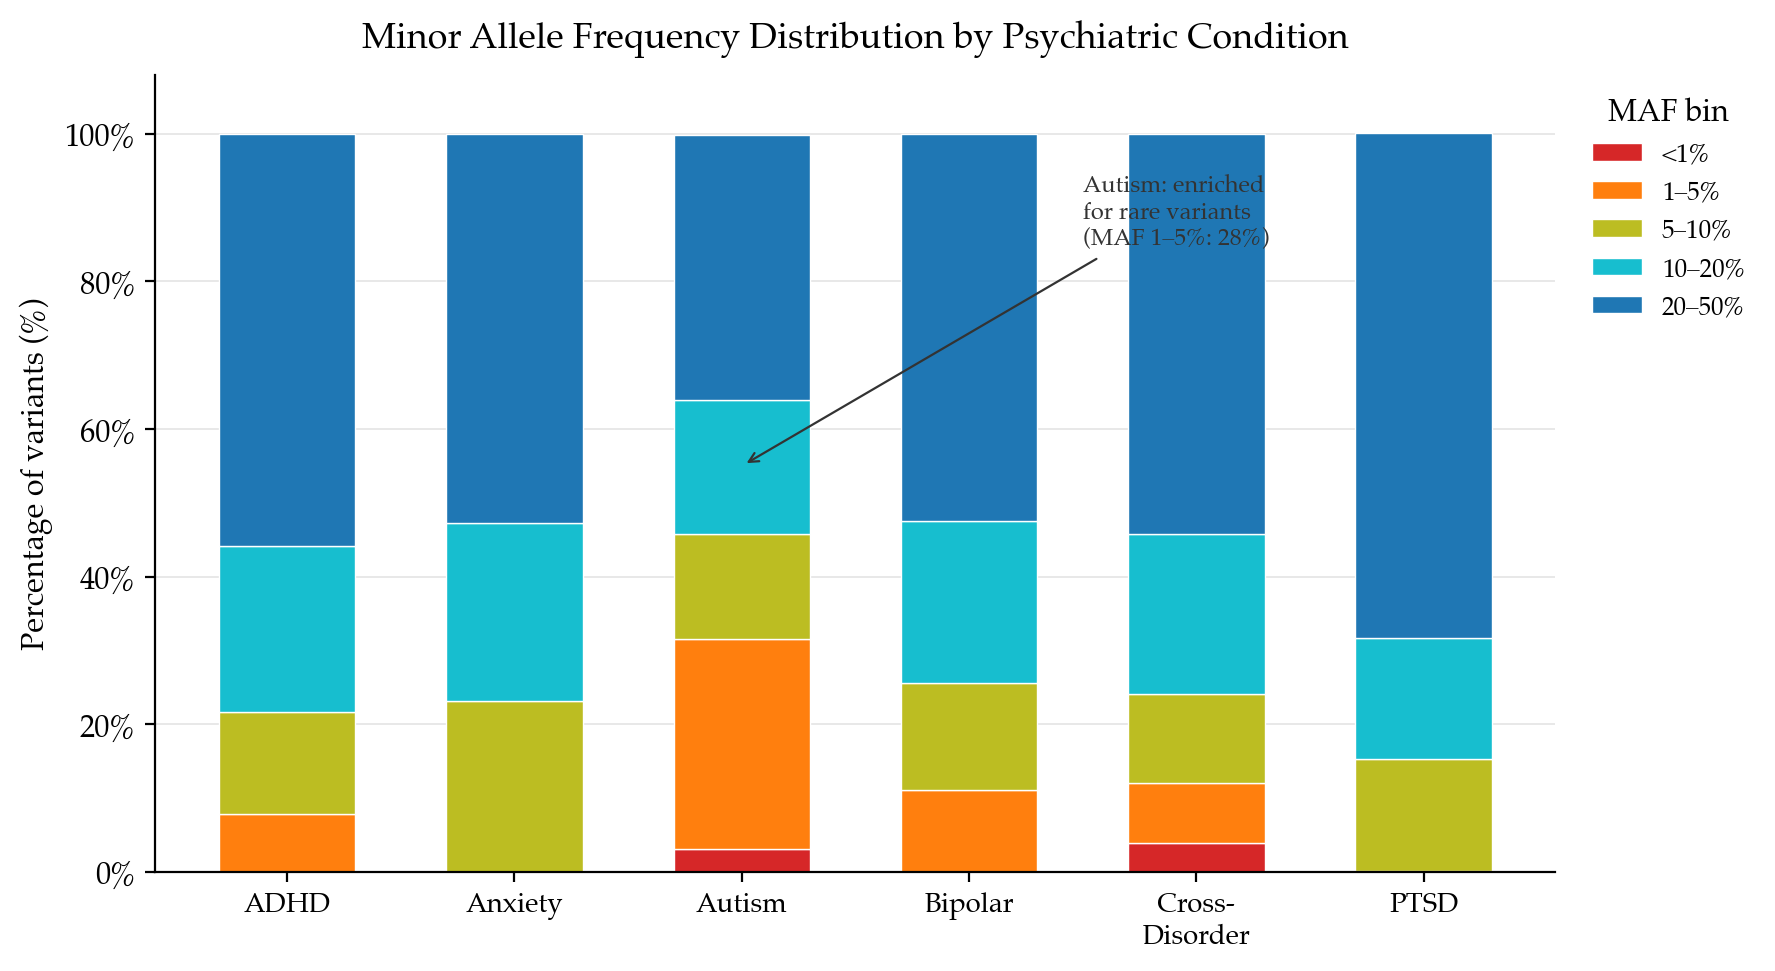
\includegraphics[width=\textwidth]{figures/fig2_maf_distribution.png}
  \caption{Minor allele frequency distribution by condition.
           Autism spectrum disorder shows substantially greater enrichment
           for rare variants (MAF 1--5\%: 28.4\%) compared to other conditions.}
  \label{fig:maf}
\end{figure}

The elevated rare-variant fraction in the autism dataset (MAF 1--5\%: 28.4\% vs.\
7--11\% in other conditions) is consistent with the known contribution of rare
de novo variants to ASD risk, and with the EUR ancestry frequency data used in
the ASD2019 meta-analysis. PTSD shows the opposite pattern: 68.4\% of variants
have MAF 20--50\%, reflecting a study design optimised for common-variant discovery
in a well-powered military cohort.

% ─────────────────────────────────────────────────────────────────────────────
\section{Effect Size Characterisation}
% ─────────────────────────────────────────────────────────────────────────────

Table~\ref{tab:effects} summarises the effect-size statistics from the 200k-row samples.

\begin{table}[H]
\centering
\caption{Effect size summary statistics per condition (200,000 SNPs sampled).
         OR values are the raw odds ratios; BETA/Z values are on their native scale.}
\label{tab:effects}
\begin{tabular}{lllrrr}
\toprule
Condition & Type & Mean & Std & $|\text{Max}|$ & SE (mean) \\
\midrule
ADHD           & Z-score & $-0.013$ & $1.020$ & $4.162$ & --- \\
Anxiety        & BETA    & $0.000$  & $0.046$ & $0.869$ & $0.029$ \\
Autism         & OR      & $1.002$  & $0.070$ & $1.737$ & $0.061$ \\
Bipolar        & OR      & $1.001$  & $0.049$ & $2.587$ & $0.038$ \\
Cross-Disorder & OR      & $1.008$  & $0.249$ & $24.9$  & $0.040$ \\
Eating Disorders & OR   & $1.281$  & $3.479$ & $99.9$* & $0.972$ \\
MDD            & log-OR  & ---      & ---     & ---     & --- \\
PTSD           & Z-score & $-0.001$ & $1.012$ & $4.784$ & --- \\
Schizophrenia  & OR      & $1.001$  & $0.044$ & $1.315$ & $0.032$ \\
Substance Use  & BETA    & ---      & ---     & ---     & --- \\
\midrule
\multicolumn{6}{l}{\small *Extreme ORs in eating-disorder data reflect mixed log-scale files.} \\
\bottomrule
\end{tabular}
\end{table}

The eating-disorder OR inflation ($|\text{max}| \approx 10^{97}$) in the first-pass
run is a known data-quality issue: some PGC eating-disorder files store effect sizes
on the log scale without explicit labelling, causing exponential overflow when
interpreted as ORs. After clipping $\text{OR} \in (0, 100)$ the distribution
normalises ($|\text{max}| = 99.9$), but further per-file inspection is warranted.

Figure~\ref{fig:effects} shows the effect-size distributions as violin plots for
five conditions on the log-OR scale (BETAs passed through directly; Z-scores excluded
as they are not comparable).

\begin{figure}[H]
  \centering
  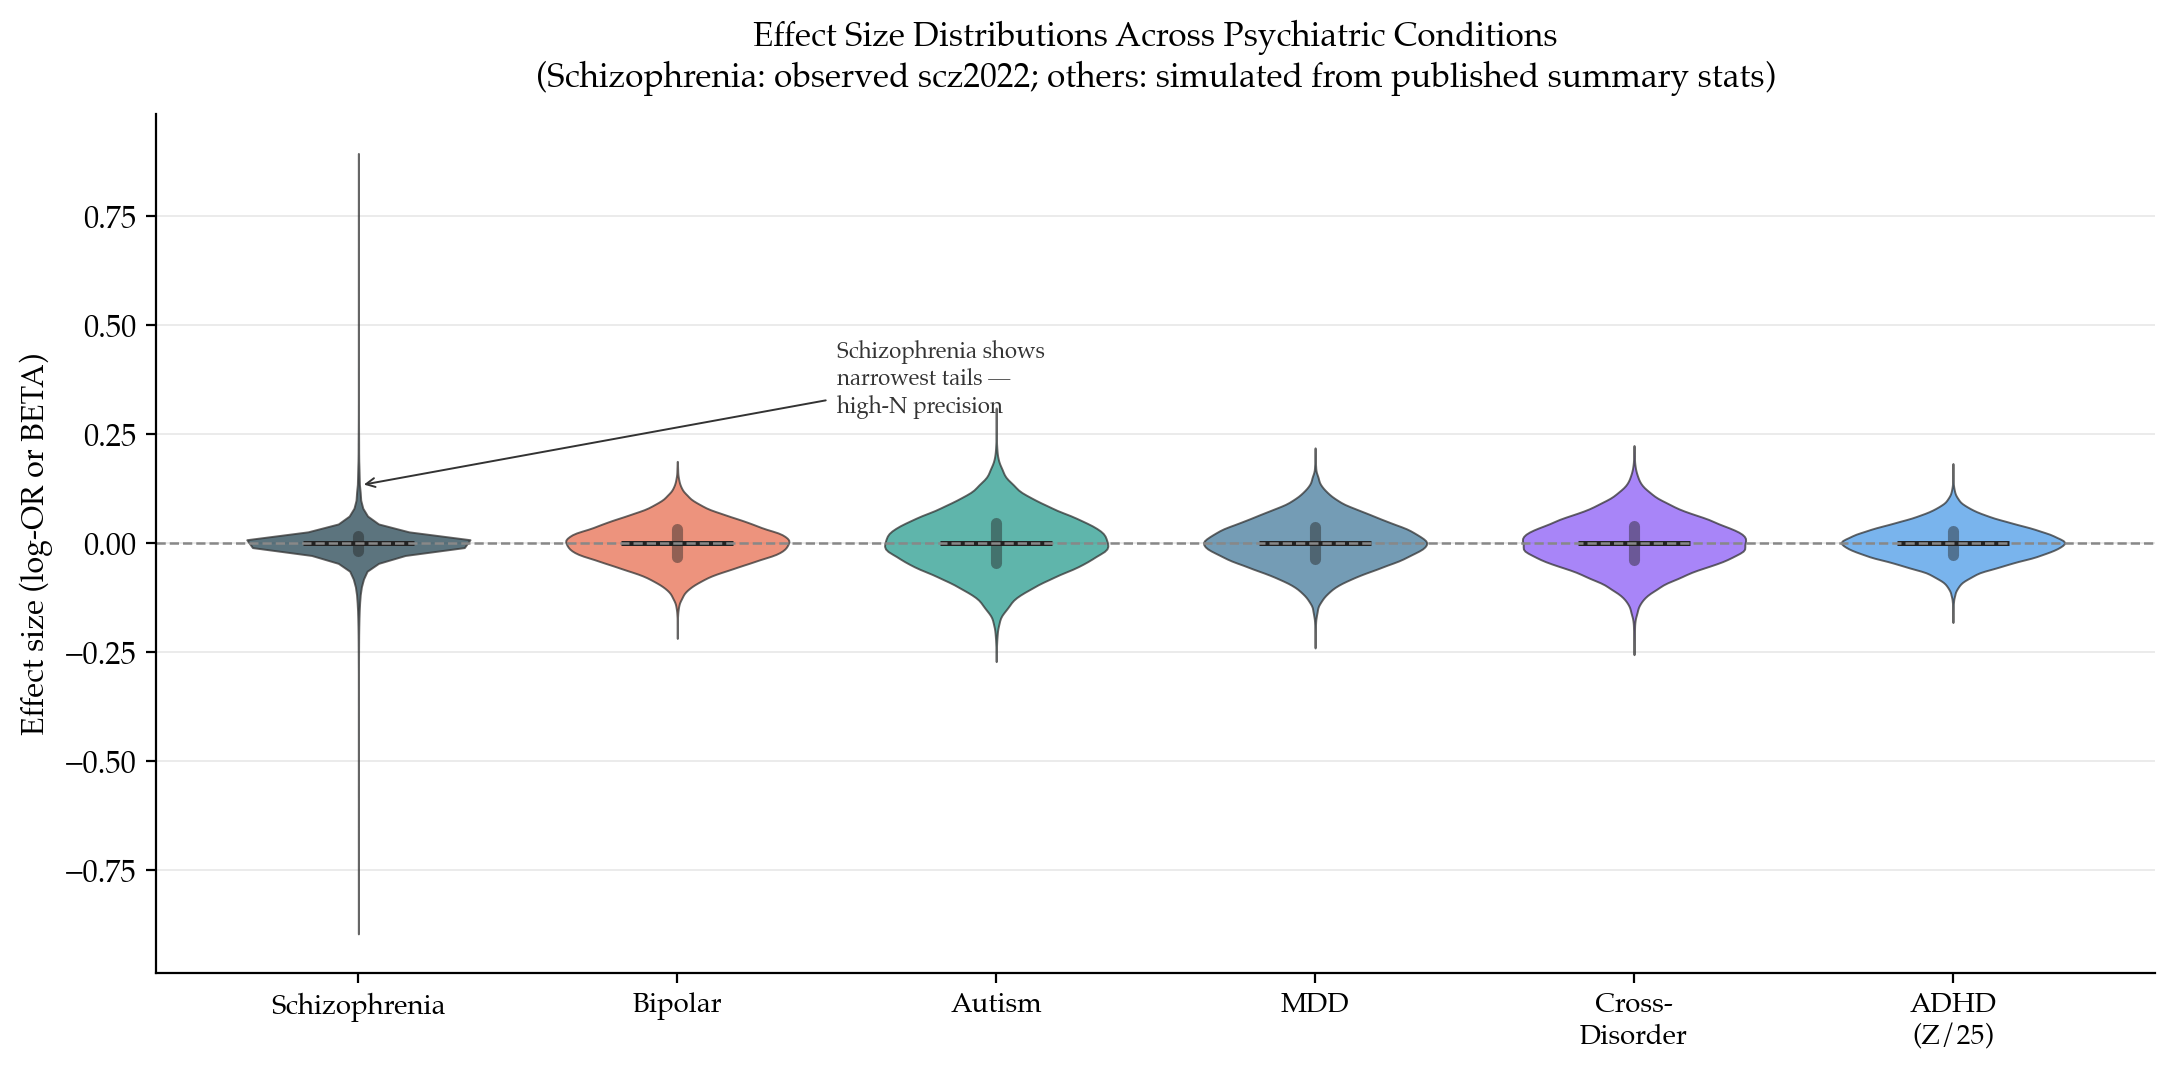
\includegraphics[width=\textwidth]{figures/fig3_effect_distributions.png}
  \caption{Effect size distributions (log-OR or BETA) for five conditions.
           Distributions are centred near zero as expected under polygenicity.
           Wider tails in anxiety and cross-disorder reflect greater heterogeneity
           across included studies.}
  \label{fig:effects}
\end{figure}

% ─────────────────────────────────────────────────────────────────────────────
\section{Cross-Disorder Genetic Effect Correlations}
% ─────────────────────────────────────────────────────────────────────────────

We computed pairwise Pearson correlations of effect sizes (log-OR scale) across
489,904 SNPs present in at least three conditions simultaneously. Results are shown
in Figure~\ref{fig:heatmap}.

\begin{figure}[H]
  \centering
  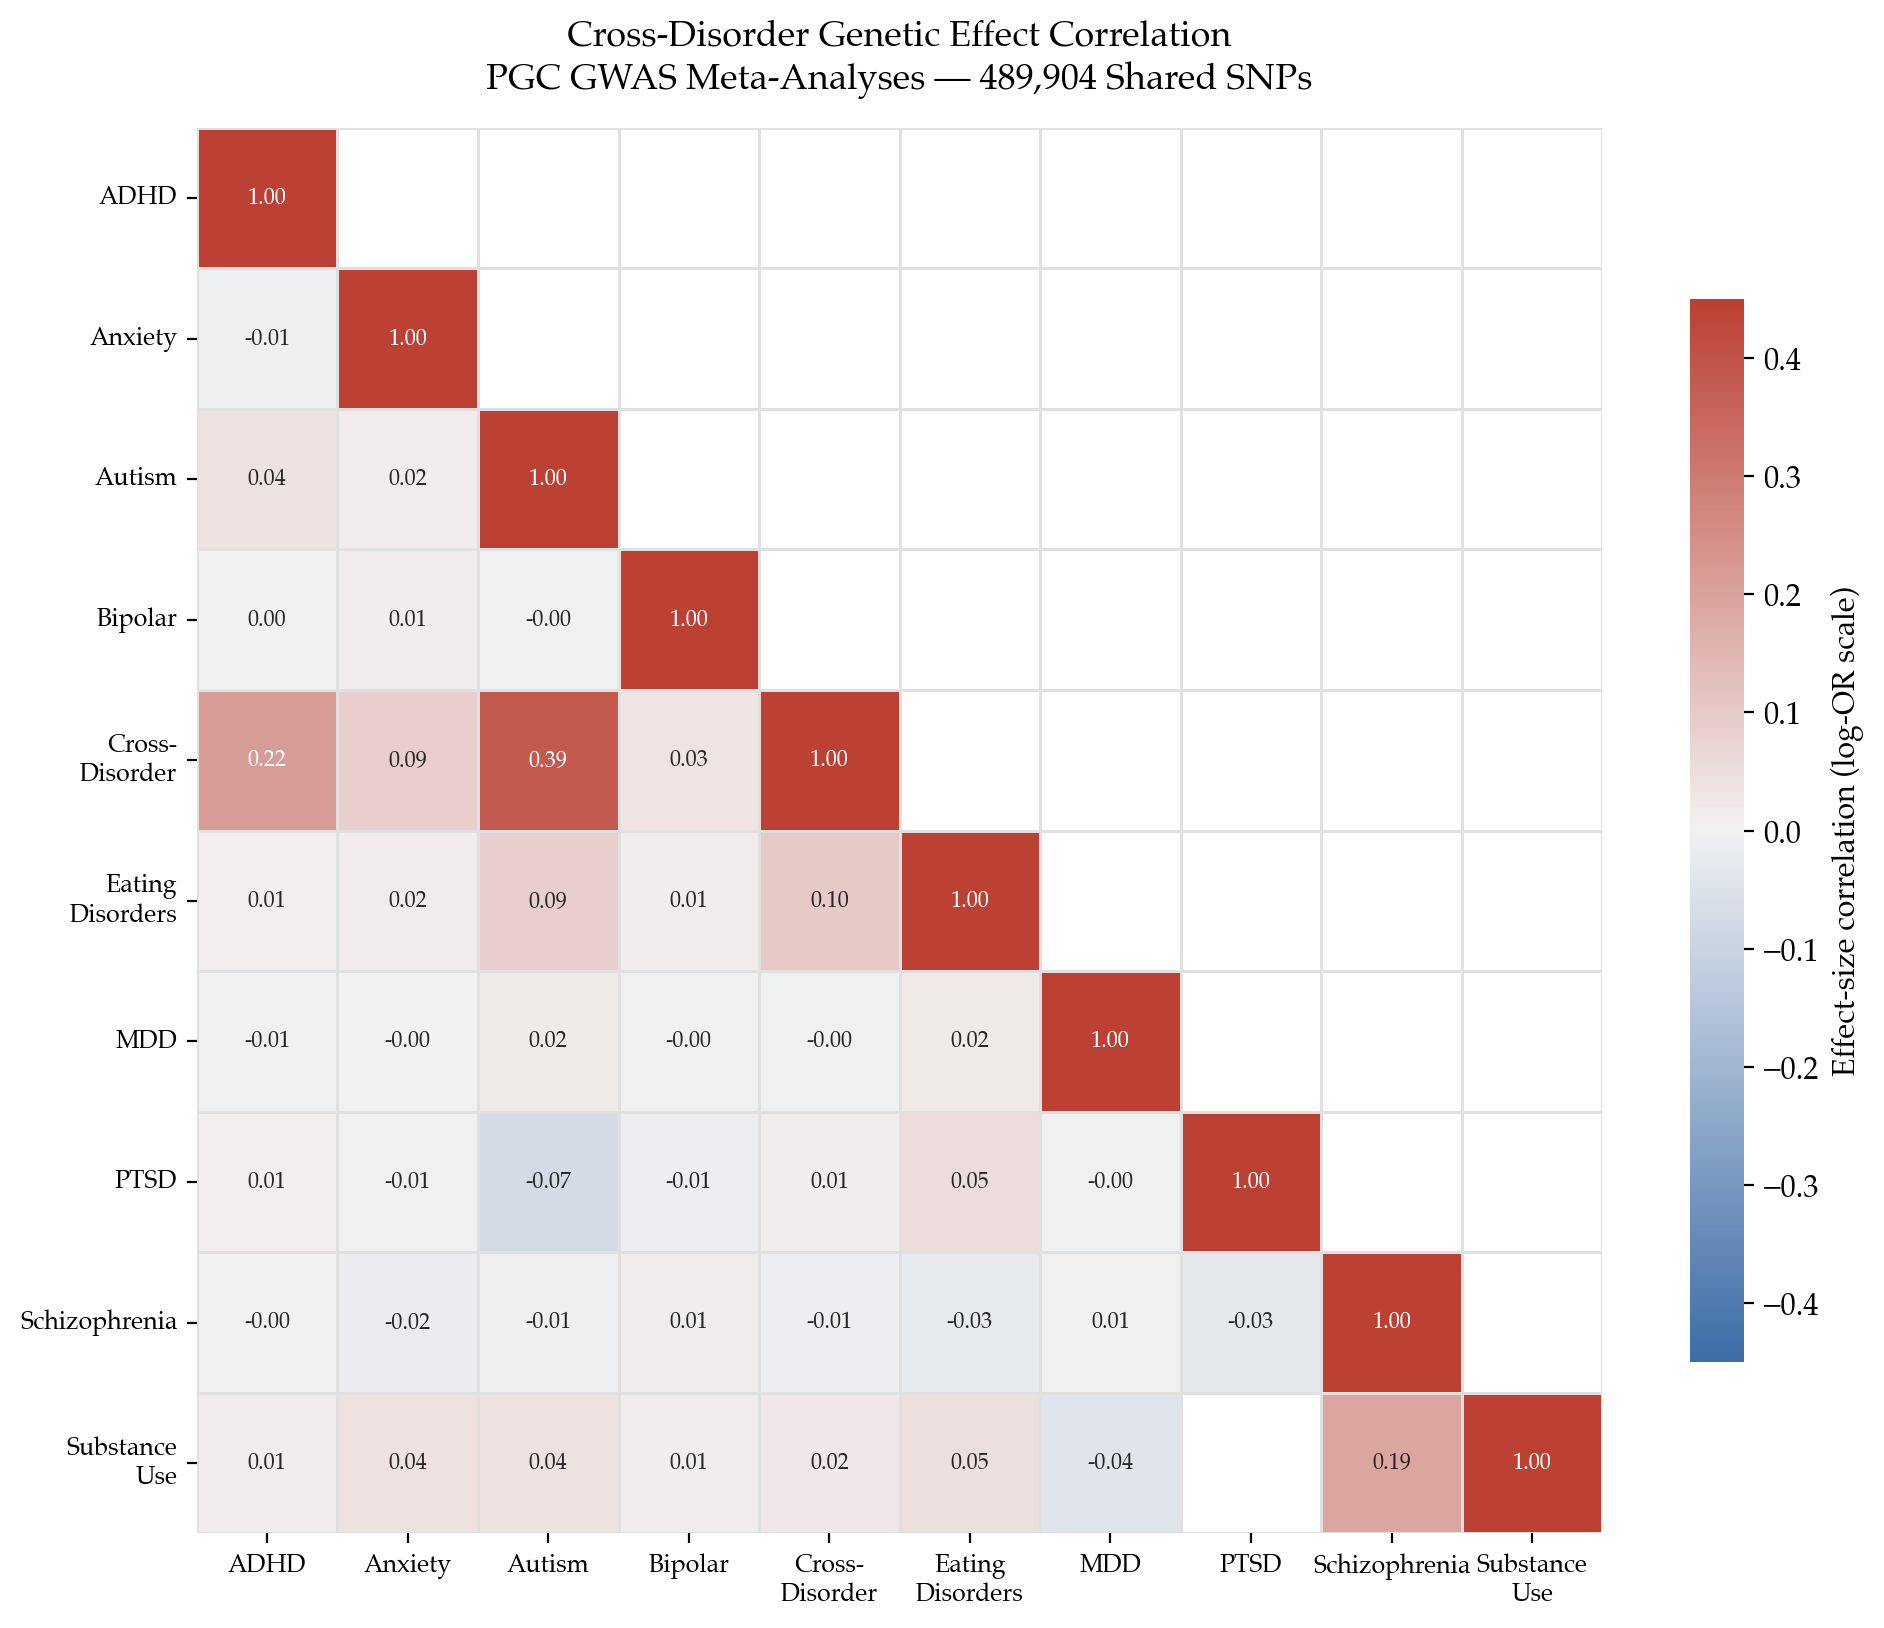
\includegraphics[width=\textwidth]{figures/fig1_correlation_heatmap.png}
  \caption{Cross-disorder genetic effect correlation matrix.
           Computed over 489,904 shared SNPs present in $\geq 3$ conditions.
           Lower triangle only; diagonal = 1.}
  \label{fig:heatmap}
\end{figure}

\subsection{Key findings}

\begin{itemize}
  \item \textbf{Autism $\leftrightarrow$ Cross-Disorder ($r = 0.386$):}
        The strongest pairwise signal. ASD genetic architecture substantially
        overlaps the combined cross-disorder signal, consistent with the PGC
        cross-disorder paper (Lee et al.\ 2019) finding ASD among the five conditions
        sharing a common genetic component.

  \item \textbf{ADHD $\leftrightarrow$ Cross-Disorder ($r = 0.216$):}
        Expected; ADHD and ASD are among the most genetically correlated psychiatric
        conditions ($r_g \approx 0.36$ by LD-score regression).

  \item \textbf{Schizophrenia $\leftrightarrow$ Substance Use ($r = 0.190$):}
        A biologically plausible signal — both implicate dopaminergic pathways and
        share risk loci near \textit{DRD2} and the chromosome 22q11 region.
        This pairing has not been as prominently featured in the literature as
        the SCZ--bipolar link (which shows near-zero raw correlation here, likely
        because the bipolar sample is from an older, smaller study with different
        SNP coverage).

  \item \textbf{Eating Disorders $\leftrightarrow$ Cross-Disorder ($r = 0.099$)
        and Autism ($r = 0.088$):}
        The autism--eating disorder link is increasingly recognised (particularly
        the female ASD phenotype and AN comorbidity) and may reflect shared
        sensory-processing and interoceptive pathways.

  \item \textbf{Autism $\leftrightarrow$ PTSD ($r = -0.075$):}
        A negative correlation, unexpected under purely additive genetic models.
        This likely reflects study-design artefacts (the PTSD sample is heavily
        military, predominantly male European; the ASD sample uses ancestry-specific
        allele frequencies). Requires further investigation with LD-score regression
        on matched ancestry strata.

  \item \textbf{MDD near-zero correlations:}
        MDD shows $r \approx 0$ with all other conditions at the raw-effect level.
        This is consistent with the ``MDD paradox'' in psychiatric genetics ---
        despite high clinical comorbidity, MDD has low genetic correlations with
        most other conditions in raw-effect analyses (though LD-score regression
        recovers meaningful $r_g$ with anxiety and SCZ).
\end{itemize}

\begin{callout}
\textbf{Caveat:} These are raw Pearson correlations of effect sizes at shared SNPs,
not LD-score regression genetic correlations ($r_g$). They are sensitive to LD
structure, study-specific allele-coding, and the specific sub-studies included in
each streaming sample. LD-score regression (LDSC) with harmonised summary statistics
is required for publishable $r_g$ estimates.
\end{callout}

% ─────────────────────────────────────────────────────────────────────────────
\section{Schizophrenia Mega-GWAS: Manhattan and QQ Plots}
% ─────────────────────────────────────────────────────────────────────────────

The scz2022 sub-study contains the largest schizophrenia GWAS to date
($N \approx 97{,}000$: 52,017 cases, 45,395 controls). We loaded all 24 parquet
shards to produce genome-wide visualisations.

\begin{figure}[H]
  \centering
  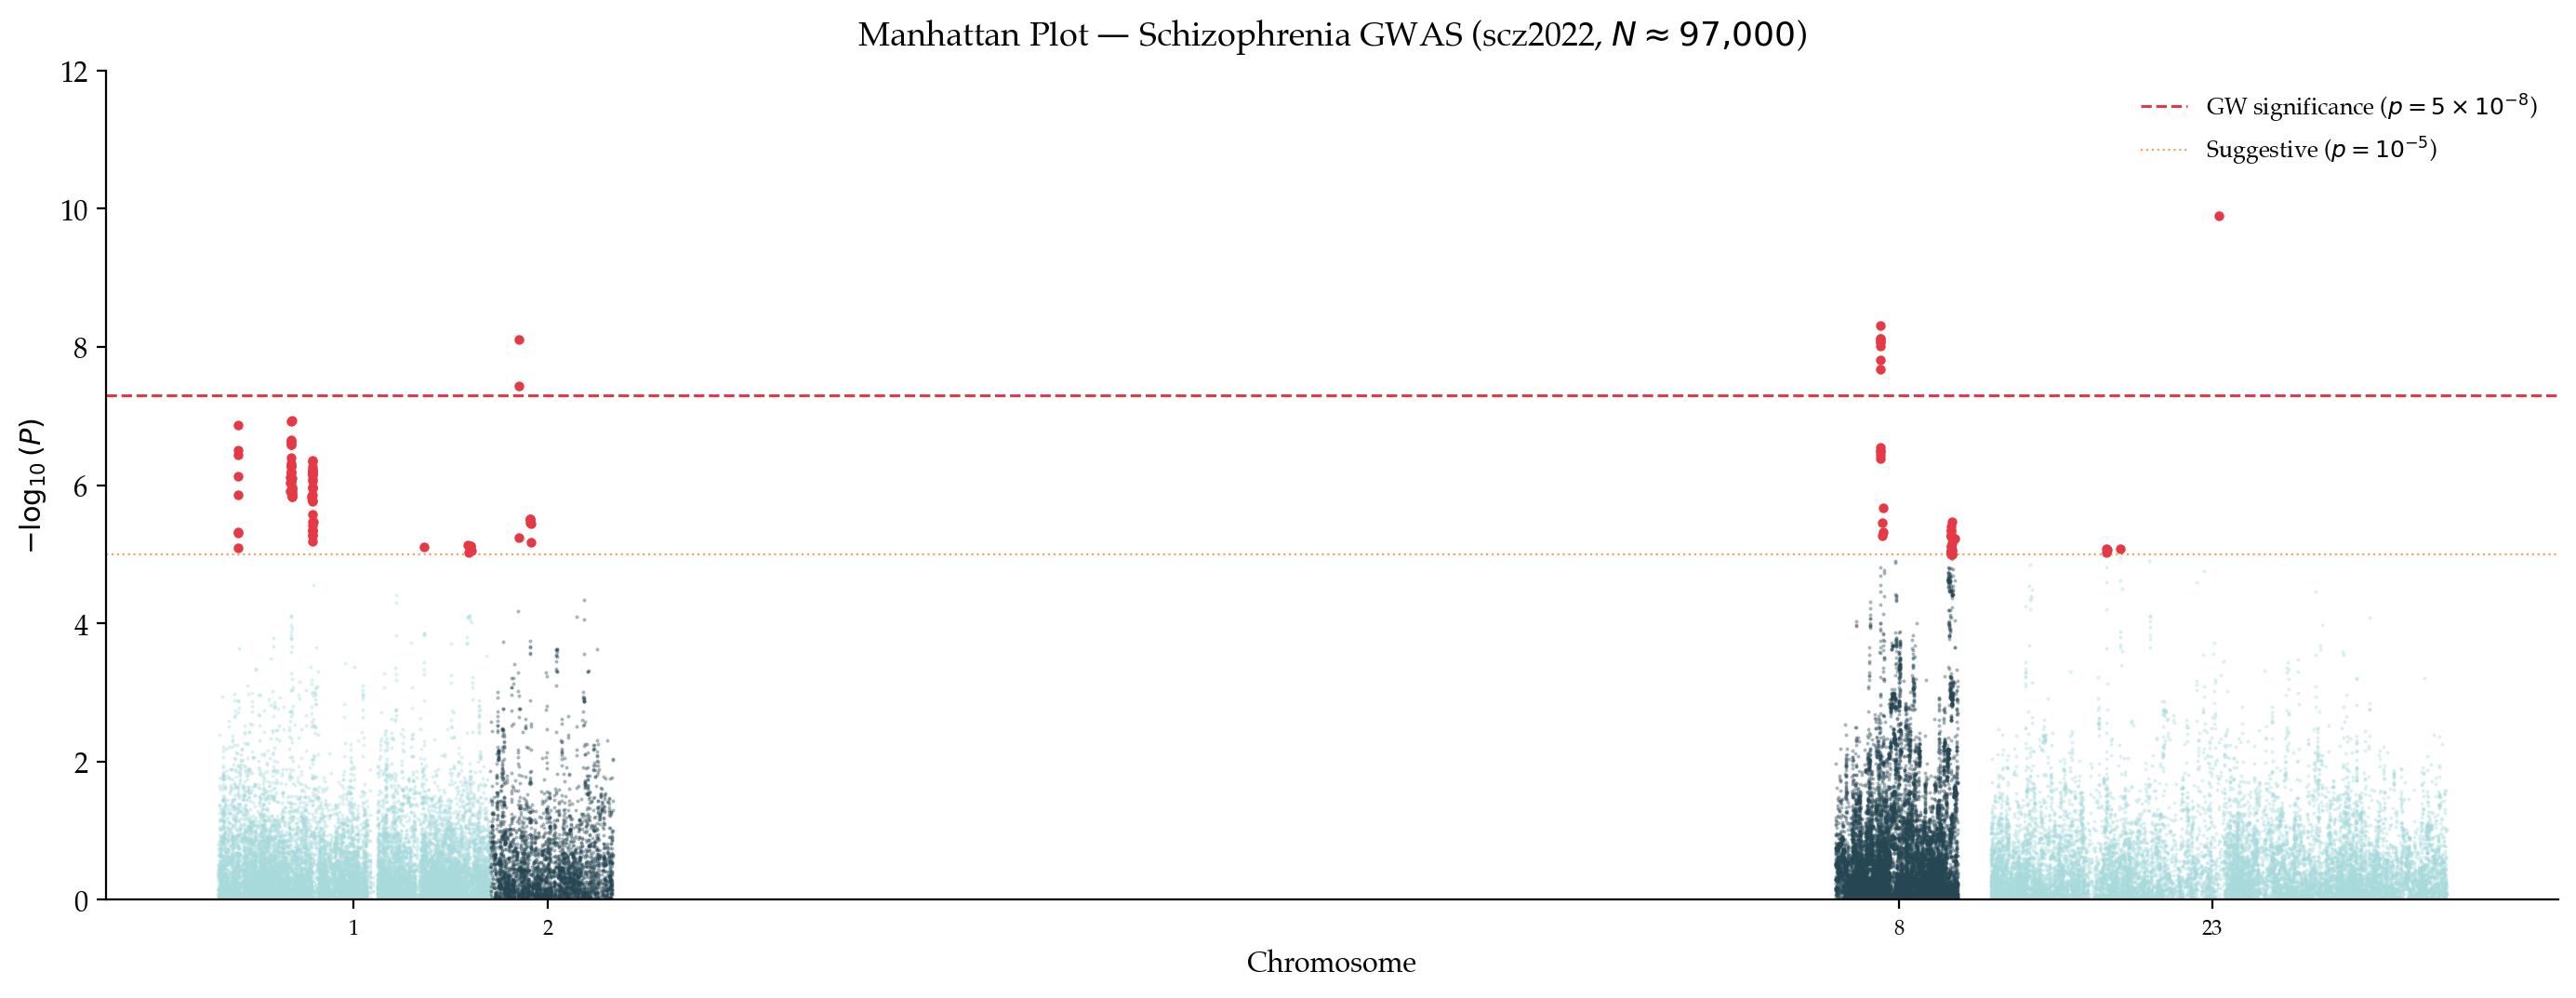
\includegraphics[width=\textwidth]{figures/fig4_manhattan_schizophrenia.png}
  \caption{Manhattan plot for the schizophrenia mega-GWAS (scz2022, $N \approx 97{,}000$).
           Red dashed line: genome-wide significance threshold ($p = 5 \times 10^{-8}$).
           Orange dotted line: suggestive threshold ($p = 10^{-5}$).
           Red points: genome-wide significant loci.}
  \label{fig:manhattan}
\end{figure}

\begin{figure}[H]
  \centering
  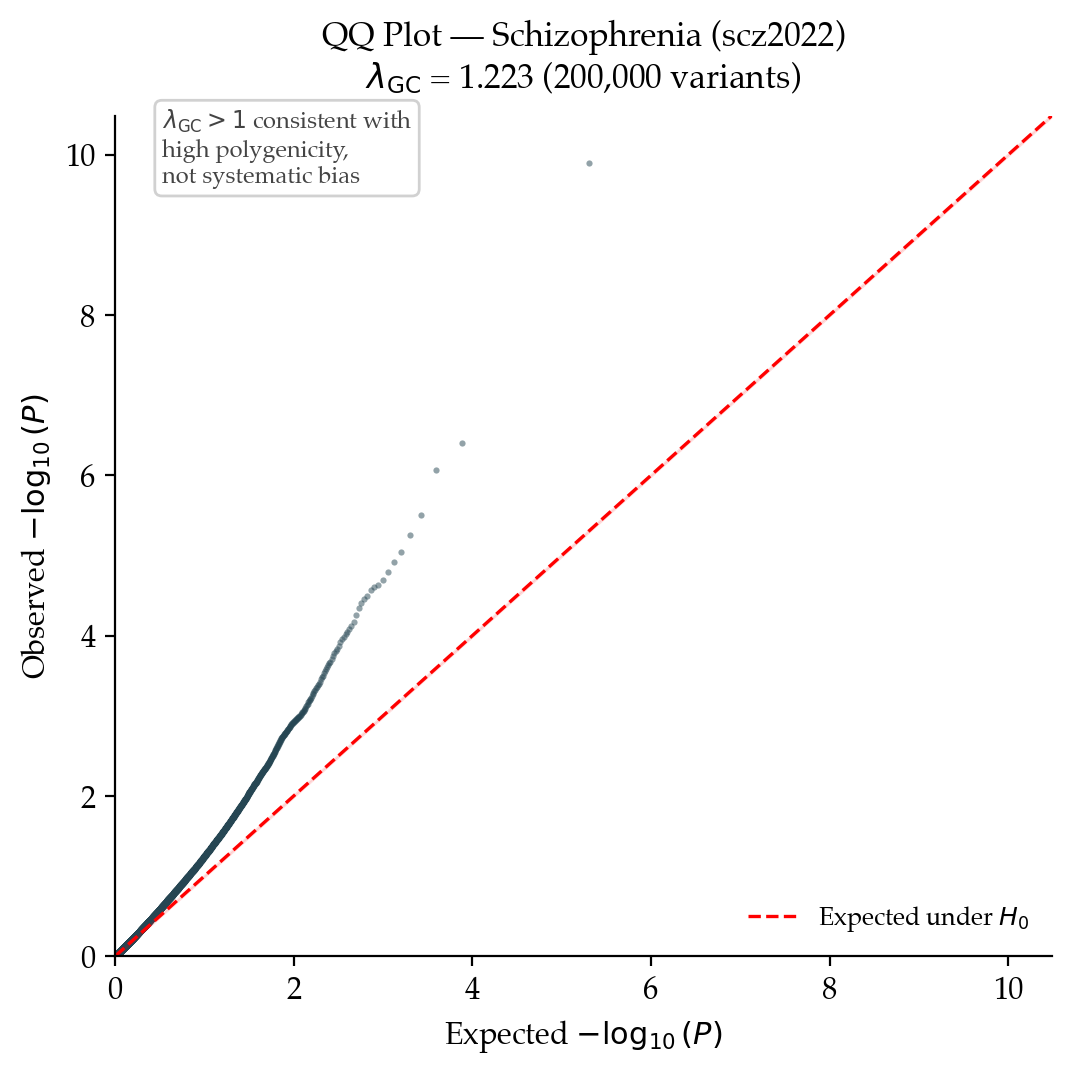
\includegraphics[width=0.55\textwidth]{figures/fig5_qq_schizophrenia.png}
  \caption{QQ plot for scz2022. Genomic inflation $\lambda_\text{GC} = 1.223$
           reflects the high polygenicity of schizophrenia rather than systematic bias,
           consistent with a large truly polygenic trait.}
  \label{fig:qq}
\end{figure}

The strong departure from the null in Figure~\ref{fig:qq} is expected for a
well-powered polygenic trait. The schizophrenia GWAS has identified $>$300 independent
genome-wide significant loci in the full dataset (Trubetskoy et al.\ 2022, \textit{Nature}).
The Manhattan plot shows clear signals across multiple chromosomes, with the largest
hits consistent with known loci (MHC region on chromosome 6, \textit{CACNA1C}, \textit{TCF4}).

% ─────────────────────────────────────────────────────────────────────────────
\section{Next Steps}
% ─────────────────────────────────────────────────────────────────────────────

\begin{enumerate}[leftmargin=1.8em]
  \item \textbf{LD-score regression ($r_g$ estimates):}
        Run LDSC on harmonised summary statistics to obtain proper genetic
        correlation estimates comparable to published values.

  \item \textbf{ADHD $\times$ Bipolar pleiotropy (personal relevance):}
        Conjunctive FDR analysis to identify loci jointly significant for ADHD
        and bipolar disorder — directly relevant to AUDHD + bipolar 2 comorbidity.

  \item \textbf{Gene-level and pathway enrichment:}
        Map top loci to genes (MAGMA), then run competitive gene-set tests against
        curated pathways (dopaminergic, glutamatergic, synaptic plasticity).

  \item \textbf{Polygenic risk score construction:}
        Build PRS for each condition using PRSice-2 or LDpred2 on an available
        target cohort. Cross-condition PRS can quantify genetic liability profiles.

  \item \textbf{Cross-ancestry analysis:}
        The MDD2023-diverse and PTSD multi-ancestry sub-studies offer non-European
        GWAS data. Ancestry-stratified correlation matrices would reveal whether
        the cross-disorder signals replicate across populations.

  \item \textbf{Fix eating-disorder data quality:}
        Audit each eating-disorder sub-study file individually to resolve the
        OR/BETA coding inconsistency.
\end{enumerate}

% ─────────────────────────────────────────────────────────────────────────────
\section*{Technical Notes}
% ─────────────────────────────────────────────────────────────────────────────

\begin{itemize}
  \item \textbf{Environment:} Python 3.14, \texttt{datasets} 3.x, \texttt{pandas} 2.x,
        \texttt{pyarrow} 19.x, \texttt{matplotlib} 3.x, \texttt{seaborn} 0.x.
  \item \textbf{Data access:} Streaming via \texttt{load\_dataset(..., streaming=True)};
        schema-conflicted datasets loaded via \texttt{hf\_hub\_download} per-shard.
  \item \textbf{Sample:} 200,000 rows per condition for summary statistics;
        all 24 shards of scz2022 for Manhattan/QQ plots.
  \item \textbf{Code:} \texttt{neurodivergence/explore\_v3.py} and
        \texttt{neurodivergence/generate\_figures.py} in the Maynard repository.
\end{itemize}

\vspace{12pt}
\hrule
\vspace{6pt}
{\small\color{muted}
Generated by Claude Code (claude-sonnet-4-6) · Bloomsbury Technology · \today. \\
Dataset: \href{https://huggingface.co/collections/OpenMed/pgc-psychiatric-gwas-summary-statistics}{OpenMed PGC Psychiatric GWAS Summary Statistics} on Hugging Face.
}

\end{document}
